% Standard model of physics
% Author: Carsten Burgard
\documentclass[border=10pt]{standalone}
%%%<
\usepackage{verbatim}
%%%>
\begin{comment}
:Title: Standard model of physics
:Tags: Styles;Decorations;Physics
:Author: Carsten Burgard
:Slug: model-physics

A standard diagram of the current standard model of physics.

In some ways, this was the ultimate, single-diagram user experience
challenge: all of our current understanding of the universe condensed
into a single infographic.

This improved diagram of the standard model of physics was made at
the CERN Webfest 2012 by David Galbraith and Carsten Burgard.

Source:
http://davidgalbraith.org/portfolio/ux-standard-model-of-the-standard-model/

Programmed in TikZ by Carsten Burgard. TikZ styles syntax by Stefan Kottwitz. 
\end{comment}

\usepackage{tikz}
\usetikzlibrary{calc,positioning,shadows.blur,decorations.pathreplacing}
\usepackage{etoolbox}

\tikzset{%
        brace/.style = { decorate, decoration={brace, amplitude=5pt} },
       mbrace/.style = { decorate, decoration={brace, amplitude=5pt, mirror} },
        label/.style = { black, midway, scale=0.5, align=center },
     toplabel/.style = { label, above=.5em, anchor=south },
    leftlabel/.style = { label,rotate=-90,left=.5em,anchor=north },   
  bottomlabel/.style = { label, below=.5em, anchor=north },
        force/.style = { rotate=-90,scale=0.4 },
        round/.style = { rounded corners=2mm },
       legend/.style = { right,scale=0.4 },
        nosep/.style = { inner sep=0pt },
   generation/.style = { anchor=base }
}

\newcommand\particle[7][white]{%
  \begin{tikzpicture}[x=1cm, y=1cm]
    \path[fill=#1,blur shadow={shadow blur steps=5}] (0.1,0) -- (0.9,0)
        arc (90:0:1mm) -- (1.0,-0.9) arc (0:-90:1mm) -- (0.1,-1.0)
        arc (-90:-180:1mm) -- (0,-0.1) arc(180:90:1mm) -- cycle;
    \ifstrempty{#7}{}{\path[fill=purple!50!white]
        (0.6,0) --(0.7,0) -- (1.0,-0.3) -- (1.0,-0.4);}
    \ifstrempty{#6}{}{\path[fill=green!50!black!50] (0.7,0) -- (0.9,0)
        arc (90:0:1mm) -- (1.0,-0.3);}
    \ifstrempty{#5}{}{\path[fill=orange!50!white] (1.0,-0.7) -- (1.0,-0.9)
        arc (0:-90:1mm) -- (0.7,-1.0);}
    \draw[\ifstrempty{#2}{dashed}{black}] (0.1,0) -- (0.9,0)
        arc (90:0:1mm) -- (1.0,-0.9) arc (0:-90:1mm) -- (0.1,-1.0)
        arc (-90:-180:1mm) -- (0,-0.1) arc(180:90:1mm) -- cycle;
    \ifstrempty{#7}{}{\node at(0.825,-0.175) [rotate=-45,scale=0.2] {#7};}
    \ifstrempty{#6}{}{\node at(0.9,-0.1)  [nosep,scale=0.17] {#6};}
    \ifstrempty{#5}{}{\node at(0.9,-0.9)  [nosep,scale=0.2] {#5};}
    \ifstrempty{#4}{}{\node at(0.1,-0.1)  [nosep,anchor=west,scale=0.25]{#4};}
    \ifstrempty{#3}{}{\node at(0.1,-0.85) [nosep,anchor=west,scale=0.3] {#3};}
    \ifstrempty{#2}{}{\node at(0.1,-0.5)  [nosep,anchor=west,scale=1.5] {#2};}
  \end{tikzpicture}
}

\begin{document}
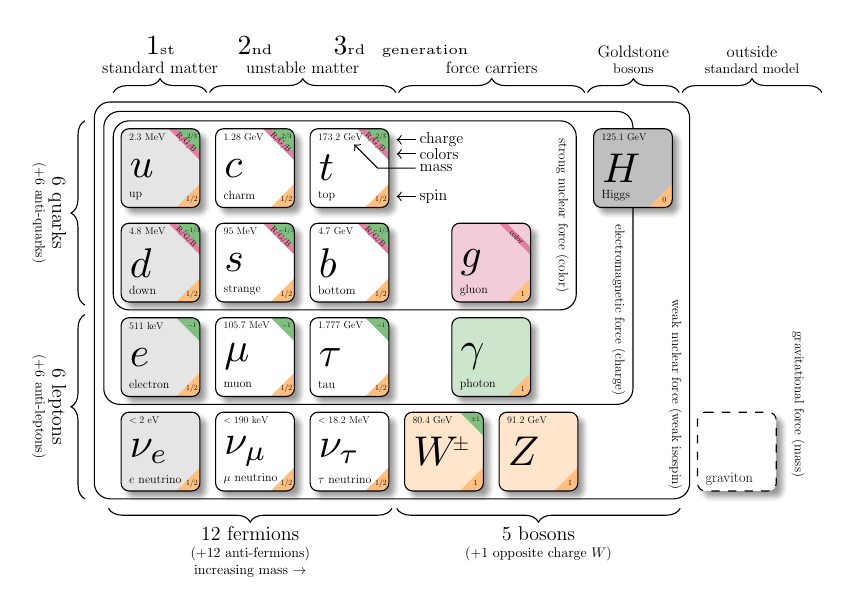
\begin{tikzpicture}[x=1.2cm, y=1.2cm]
  \draw[round] (-0.5,0.5) rectangle (4.4,-1.5);
  \draw[round] (-0.6,0.6) rectangle (5.0,-2.5);
  \draw[round] (-0.7,0.7) rectangle (5.6,-3.5);

  \node at(0, 0)   {\particle[gray!20!white]
                   {$u$}        {\Large up}       {\Large $2.3$ MeV}{\Large 1/2}{\Large $2/3$}{\Large R/G/B}};
  \node at(0,-1)   {\particle[gray!20!white]
                   {$d$}        {\Large down}    {\Large $4.8$ MeV}{\Large 1/2}{\Large $-1/3$}{\Large R/G/B}};
  \node at(0,-2)   {\particle[gray!20!white]
                   {$e$}        {\Large electron}       {\Large $511$ keV}{\Large 1/2}{\Large $-1$}{}};
  \node at(0,-3)   {\particle[gray!20!white]
                   {$\nu_e$}    {\Large $e$ neutrino}         {\Large $<2$ eV}{\Large 1/2}{}{}};
  \node at(1, 0)   {\particle
                   {$c$}        {\Large charm}   {\Large $1.28$ GeV}{\Large 1/2}{\Large $2/3$}{\Large R/G/B}};
  \node at(1,-1)   {\particle 
                   {$s$}        {\Large strange}  {\Large $95$ MeV}{\Large 1/2}{\Large $-1/3$}{\Large R/G/B}};
  \node at(1,-2)   {\particle
                   {$\mu$}      {\Large muon}         {\Large $105.7$ MeV}{\Large 1/2}{\Large $-1$}{}};
  \node at(1,-3)   {\particle
                   {$\nu_\mu$}  {\Large $\mu$ neutrino}    {\Large $<190$ keV}{\Large 1/2}{}{}};
  \node at(2, 0)   {\particle
                   {$t$}        {\Large top}    {\Large $173.2$ GeV}{\Large 1/2}{\Large $2/3$}{\Large R/G/B}};
  \node at(2,-1)   {\particle
                   {$b$}        {\Large bottom}  {\Large $4.7$ GeV}{\Large 1/2}{\Large $-1/3$}{\Large  R/G/B}};
  \node at(2,-2)   {\particle
                   {$\tau$}     {\Large tau}          {\Large $1.777$ GeV}{\Large 1/2}{\Large $-1$}{}};
  \node at(2,-3)   {\particle
                   {$\nu_\tau$} {\Large $\tau$ neutrino}  {\Large $<18.2$ MeV}{\Large 1/2}{}{}};
  \node at(3,-3)   {\particle[orange!20!white]
                   {$W^{\hspace{-.3ex}\scalebox{.5}{$\pm$}}$}
                                {}              {\Large $80.4$ GeV}{\Large 1}{\Large $\pm1$}{}};
  \node at(4,-3)   {\particle[orange!20!white]
                   {$Z$}        {}                    {\Large $91.2$ GeV}{\Large 1}{}{}};
  \node at(3.5,-2) {\particle[green!50!black!20]
                   {$\gamma$}   {\Large photon}                        {}{\Large 1}{}{}};
  \node at(3.5,-1) {\particle[purple!20!white]
                   {$g$}        {\Large gluon}                    {}{\Large 1}{}{\Large color}};
  \node at(5,0)    {\particle[gray!50!white]
                   {$H$}        {\Large Higgs}              {\Large $125.1$ GeV}{\Large 0}{}{}};
  \node at(6.1,-3) {\particle
                   {}           {\LARGE \textcolor{black} {graviton}}                       {}{}{}{}};

  \node at(4.25,-0.5) [force] {\large strong nuclear force (color)};
  \node at(4.85,-1.5) [force] {\large electromagnetic force (charge)};
  \node at(5.45,-2.4) [force] {\large weak nuclear force (weak isospin)};
  \node at(6.75,-2.5) [force] {\large gravitational force (mass)};

  \draw [<-] (2.5,0.3)   -- (2.7,0.3)          node [legend] {\Large charge};
  \draw [<-] (2.5,0.15)  -- (2.7,0.15)         node [legend] {\Large colors};
  \draw [<-] (2.05,0.25) -- (2.3,0) -- (2.7,0) node [legend] {\Large mass};
  \draw [<-] (2.5,-0.3)  -- (2.7,-0.3)         node [legend] {\Large spin};

  \draw [mbrace] (-0.8,0.5)  -- (-0.8,-1.45)
                 node[leftlabel] {\Large  6 quarks\\(+6 anti-quarks)};
  \draw [mbrace] (-0.8,-1.55) -- (-0.8,-3.5)
                 node[leftlabel] {\Large  6 leptons\\(+6 anti-leptons)};
  \draw [mbrace] (-0.55,-3.6) -- (2.45,-3.6)
                 node[bottomlabel]
                 {\Large 12 fermions\\(+12 anti-fermions)\\increasing mass $\to$};
  \draw [mbrace] (2.5,-3.6) -- (5.5,-3.6)
                 node[bottomlabel] {\Large 5 bosons\\(+1 opposite charge $W$)};

  \draw [brace] (-0.5,.8) -- (0.49,.8) node[toplabel]         {\large standard matter};
  \draw [brace] (0.52,.8)  -- (2.49,.8) node[toplabel]         {\large unstable matter};
  \draw [brace] (2.52,.8)  -- (4.49,.8) node[toplabel]          {\large force carriers};
  \draw [brace] (4.52,.8)  -- (5.49,.8) node[toplabel]       {\large Goldstone\\bosons};
  \draw [brace] (5.52,.8)  -- (7,.8)   node[toplabel] {\large outside\\standard model};

  \node at (0,1.2)   [generation] {1\tiny st};
  \node at (1,1.2)   [generation] {2\tiny nd};
  \node at (2,1.2)   [generation] {3\tiny rd};
  \node at (2.8,1.2) [generation] {\tiny generation};
\end{tikzpicture}
\end{document}
